\section{State of the art}

\todo{lavori simili}
Nel corso degli anni diversi studi hanno provato ad affrontare la questione usando metodi che portassero ad ottenere dei modelli statistici in grado di capire e modellare le relazioni tra inquinanti e condizioni atmosferiche e, indipendentemente dal metodo usato, si è visto come variabili legate alla meteorologia, all’altezza dello strato di rimescolamento ed alla stagionalità siano in grado di spiegare con una certa precisioni gli andamenti delle serie di inquinanti. Segal ha dimostrato come fosse possibile applicare un modello numerico per simulare la circolazione di aria nella zona della baia di Chesapake (USA) per poterne predirre la qualità dell’aria [32]. Eagleman nel suo libro illustra diversi metodi matematici applicabili per lo studio delle concentrazioni di inquinanti e degli effetti che ha su di esse la meteorologia [10]. Aldrin e Haff propongono un modello per la stima delle concentrazioni dei principali inquinanti utilizzando i valori delle variabili meteorologiche e dei volumi di traffico [2]. Un altro studio si è invece concentrato sull’influenza della meteorologia sul PM10 e su come essa complichi l’analisi dei reali trend di un inquinante [4]. Cattani, in uno studio del 2014, ha proposto un metodo matematico per il calcolo dei trend delle concentrazioni di un inquinante, eliminando l’influenza della stagionalità 
%mbelotti: rivedere, si potrebbe articolare meglio

\todo{approfondimento da introduzione}

\todo{inventario INEMAR ecc.}
Informations about emissions trends, fuel usage and individual sectors' contributions to each pollutant were gathered from the national and regional air quality inventories. \cite{iir2020, inemar2017}

\todo{trend ecc.}
%questi sono i grafici dei trend dei principali inquinanti nei periodi considerati per ciascuno durante la generazione delle serie normalizzate, ovviamente sono da organizzare meglio
\begin{figure}
\centering
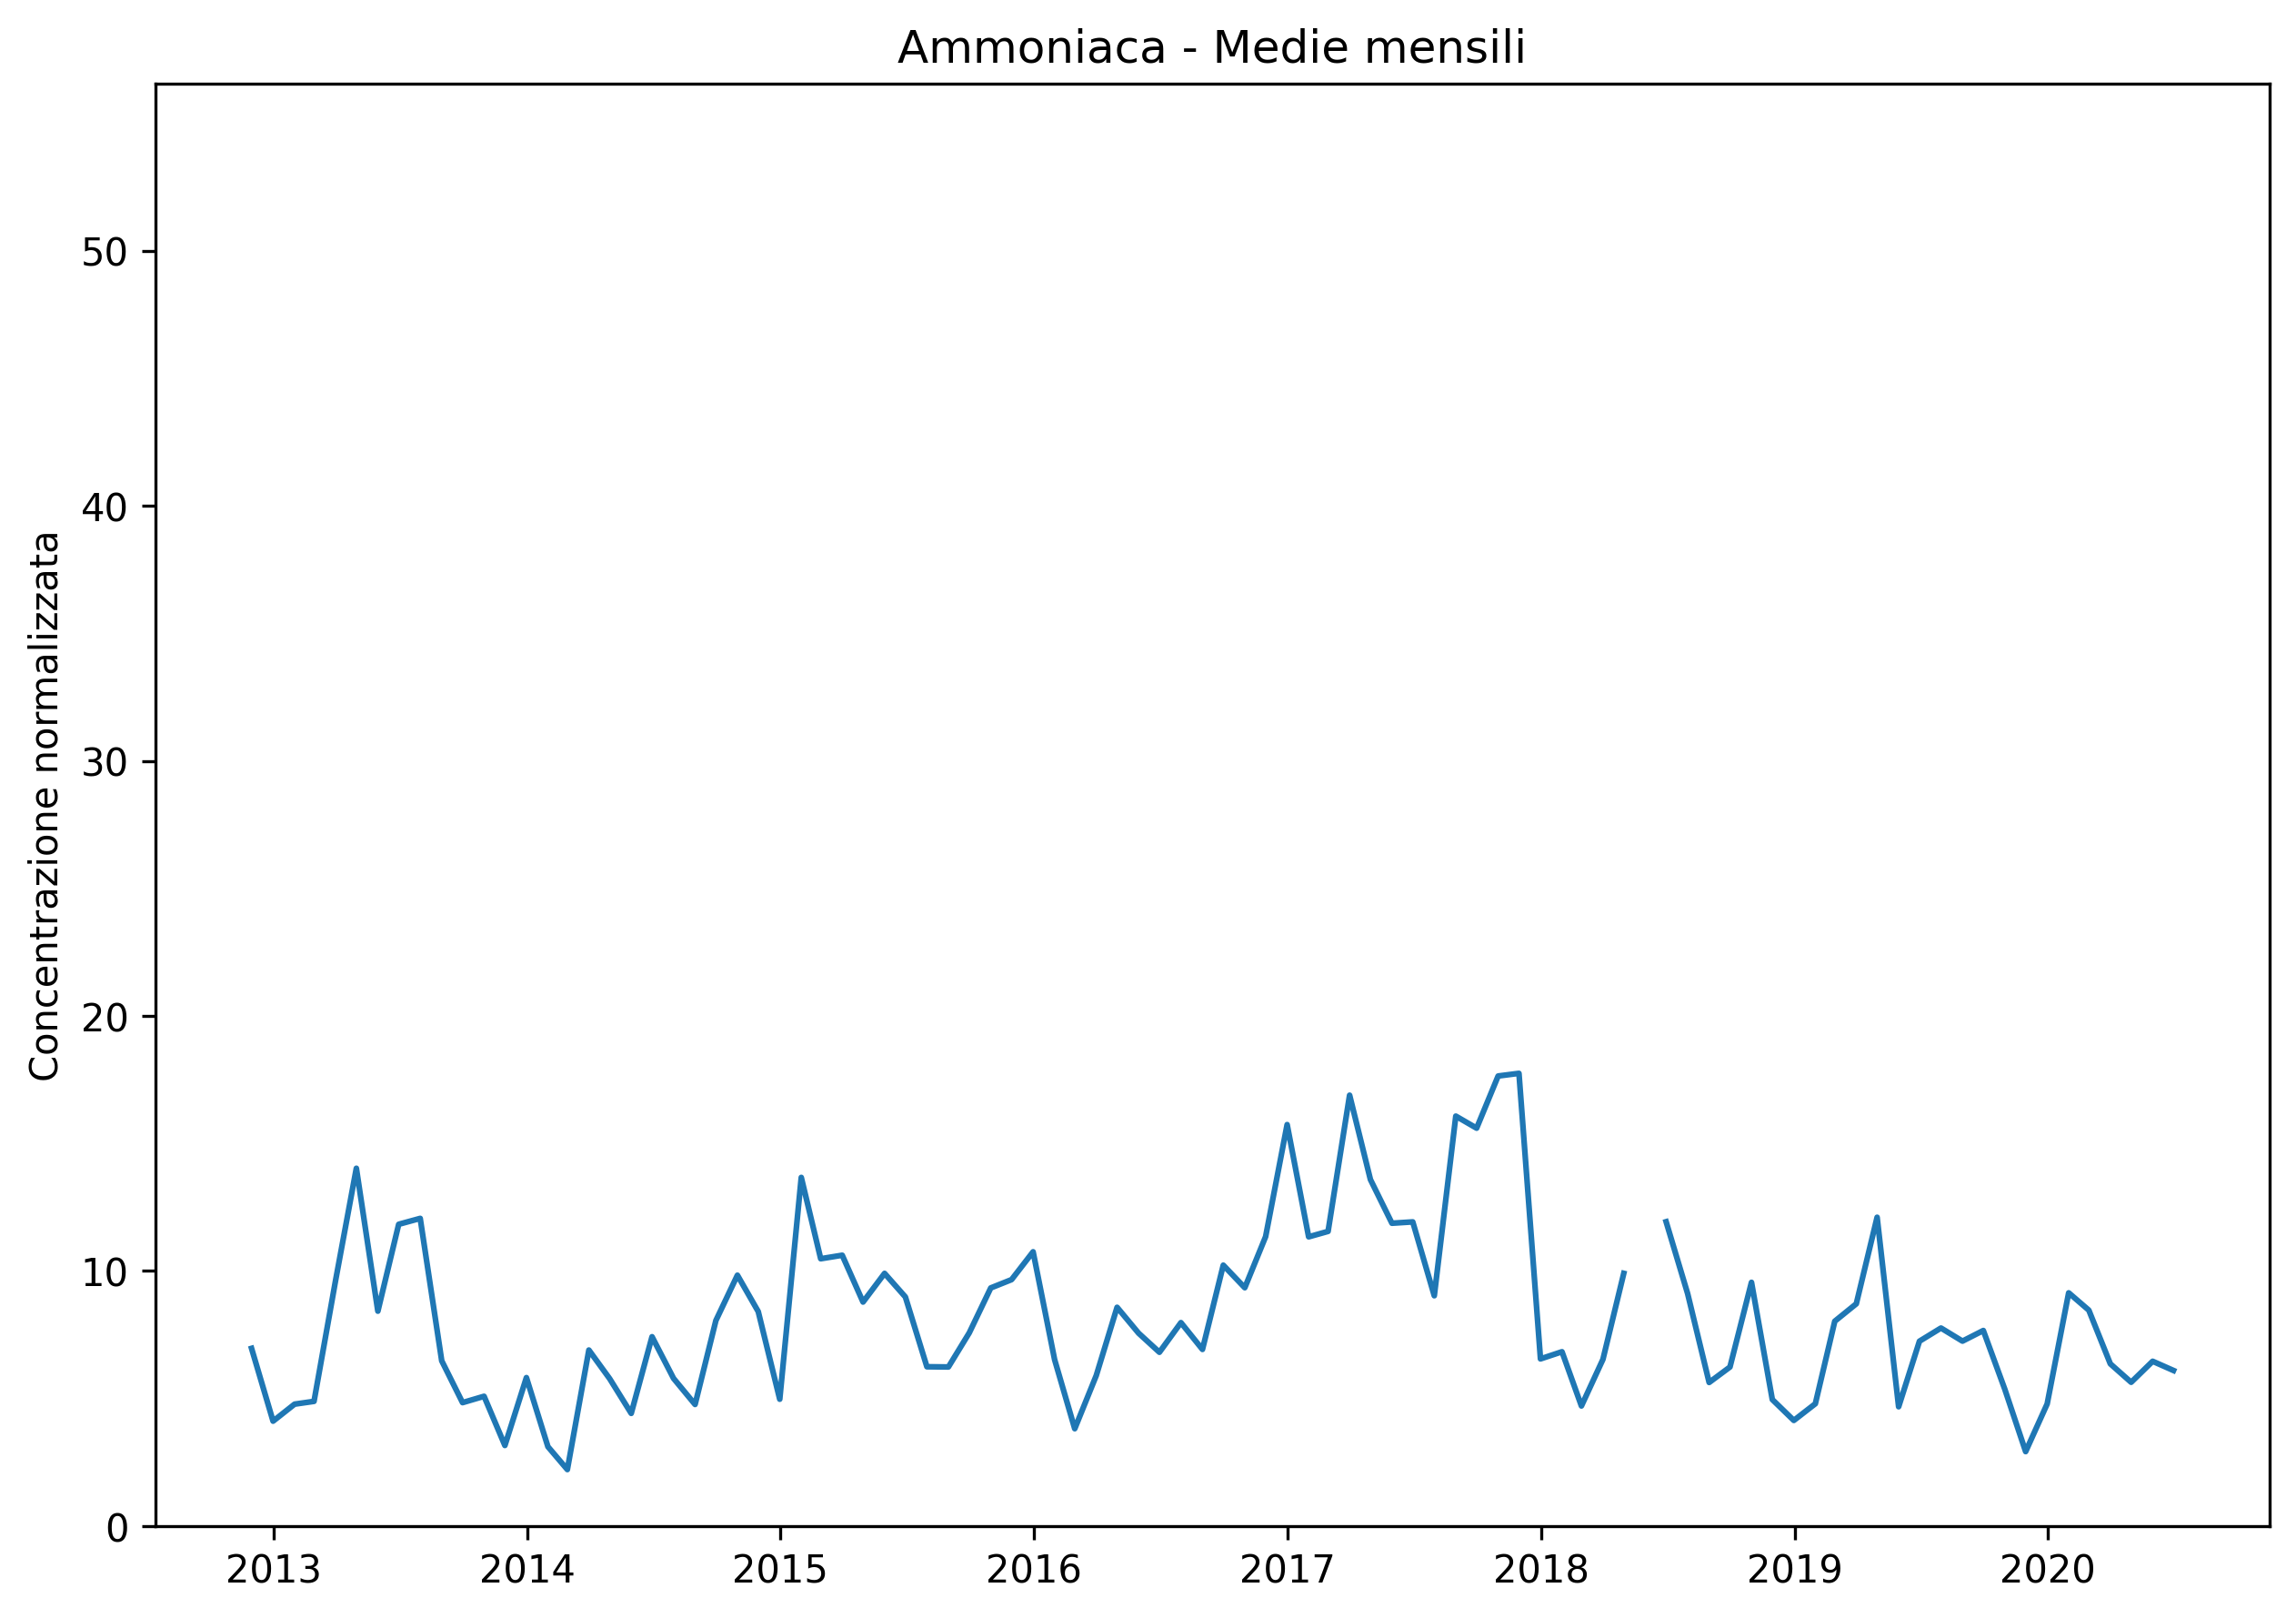
\includegraphics[width=0.75\textwidth]{Ammoniaca_medie_mensili}
\caption{Medie mensili ammoniaca}
\label{fig:ammoniaca_medie_mensili_reali}
\end{figure}


\begin{figure}
\centering
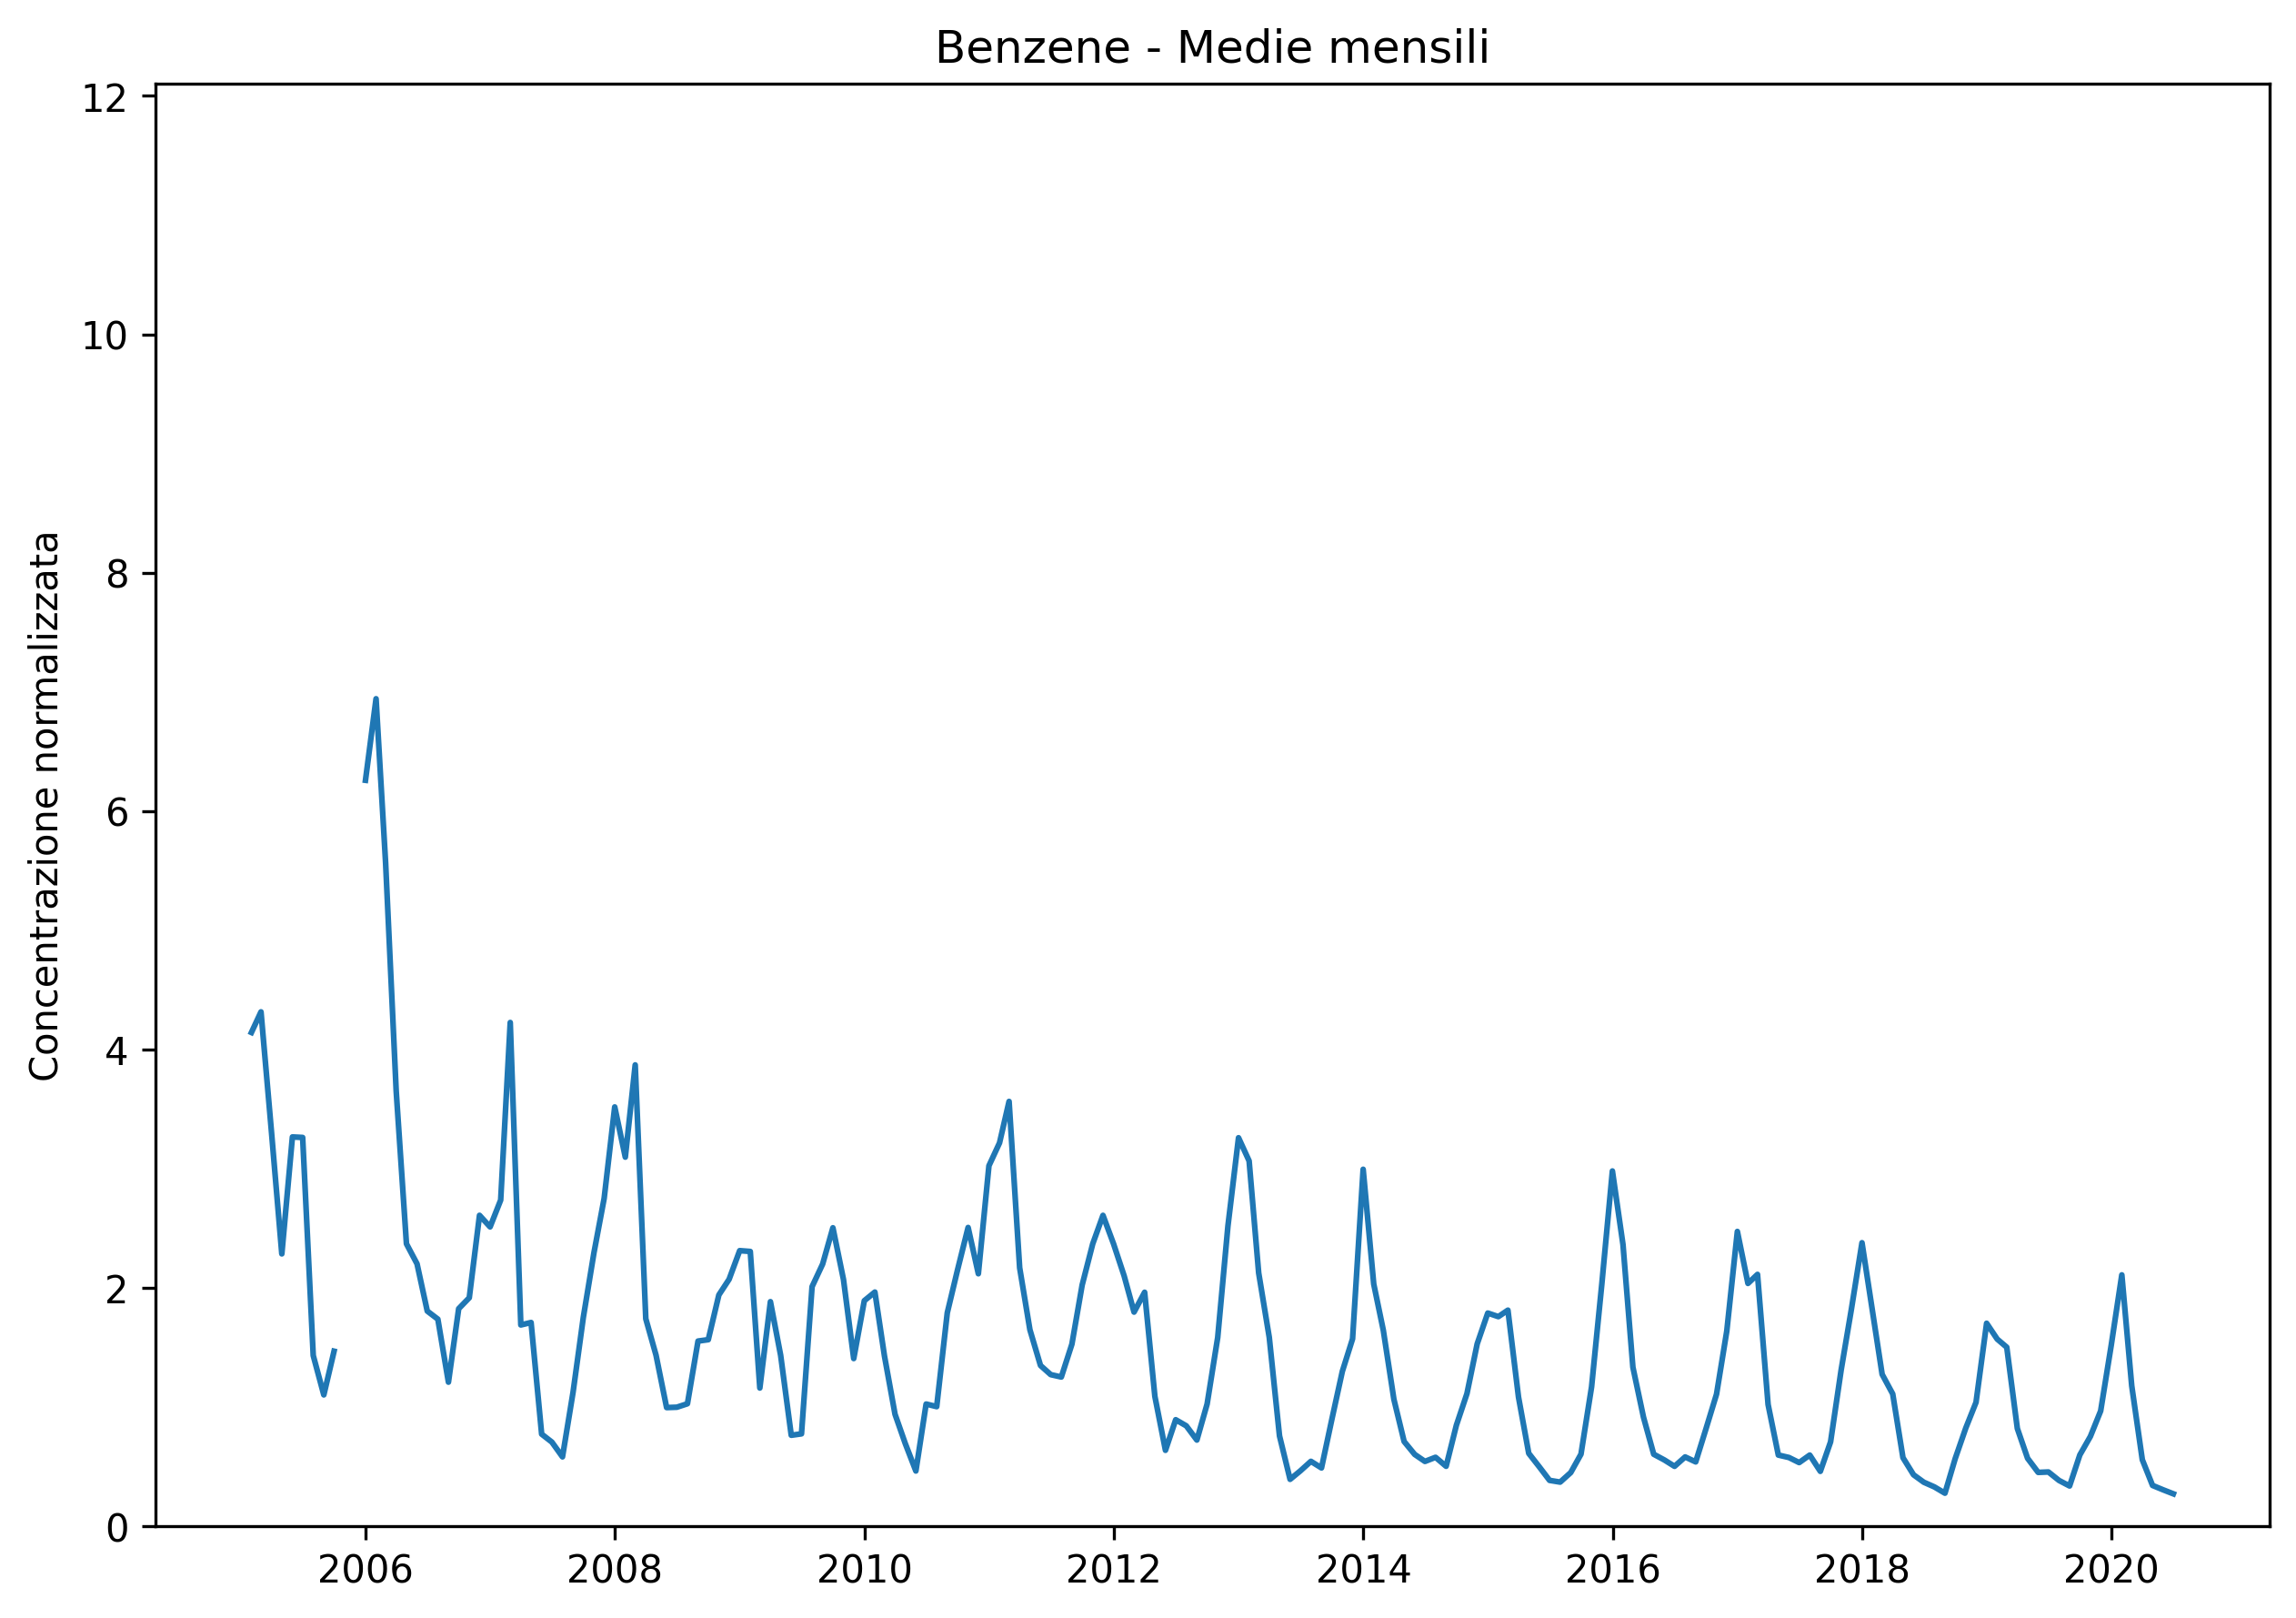
\includegraphics[width=0.75\textwidth]{Benzene_medie_mensili}
\caption{Medie mensili benzene}
\label{fig:benzene_medie_mensili_reali}
\end{figure}

\begin{figure}
\centering
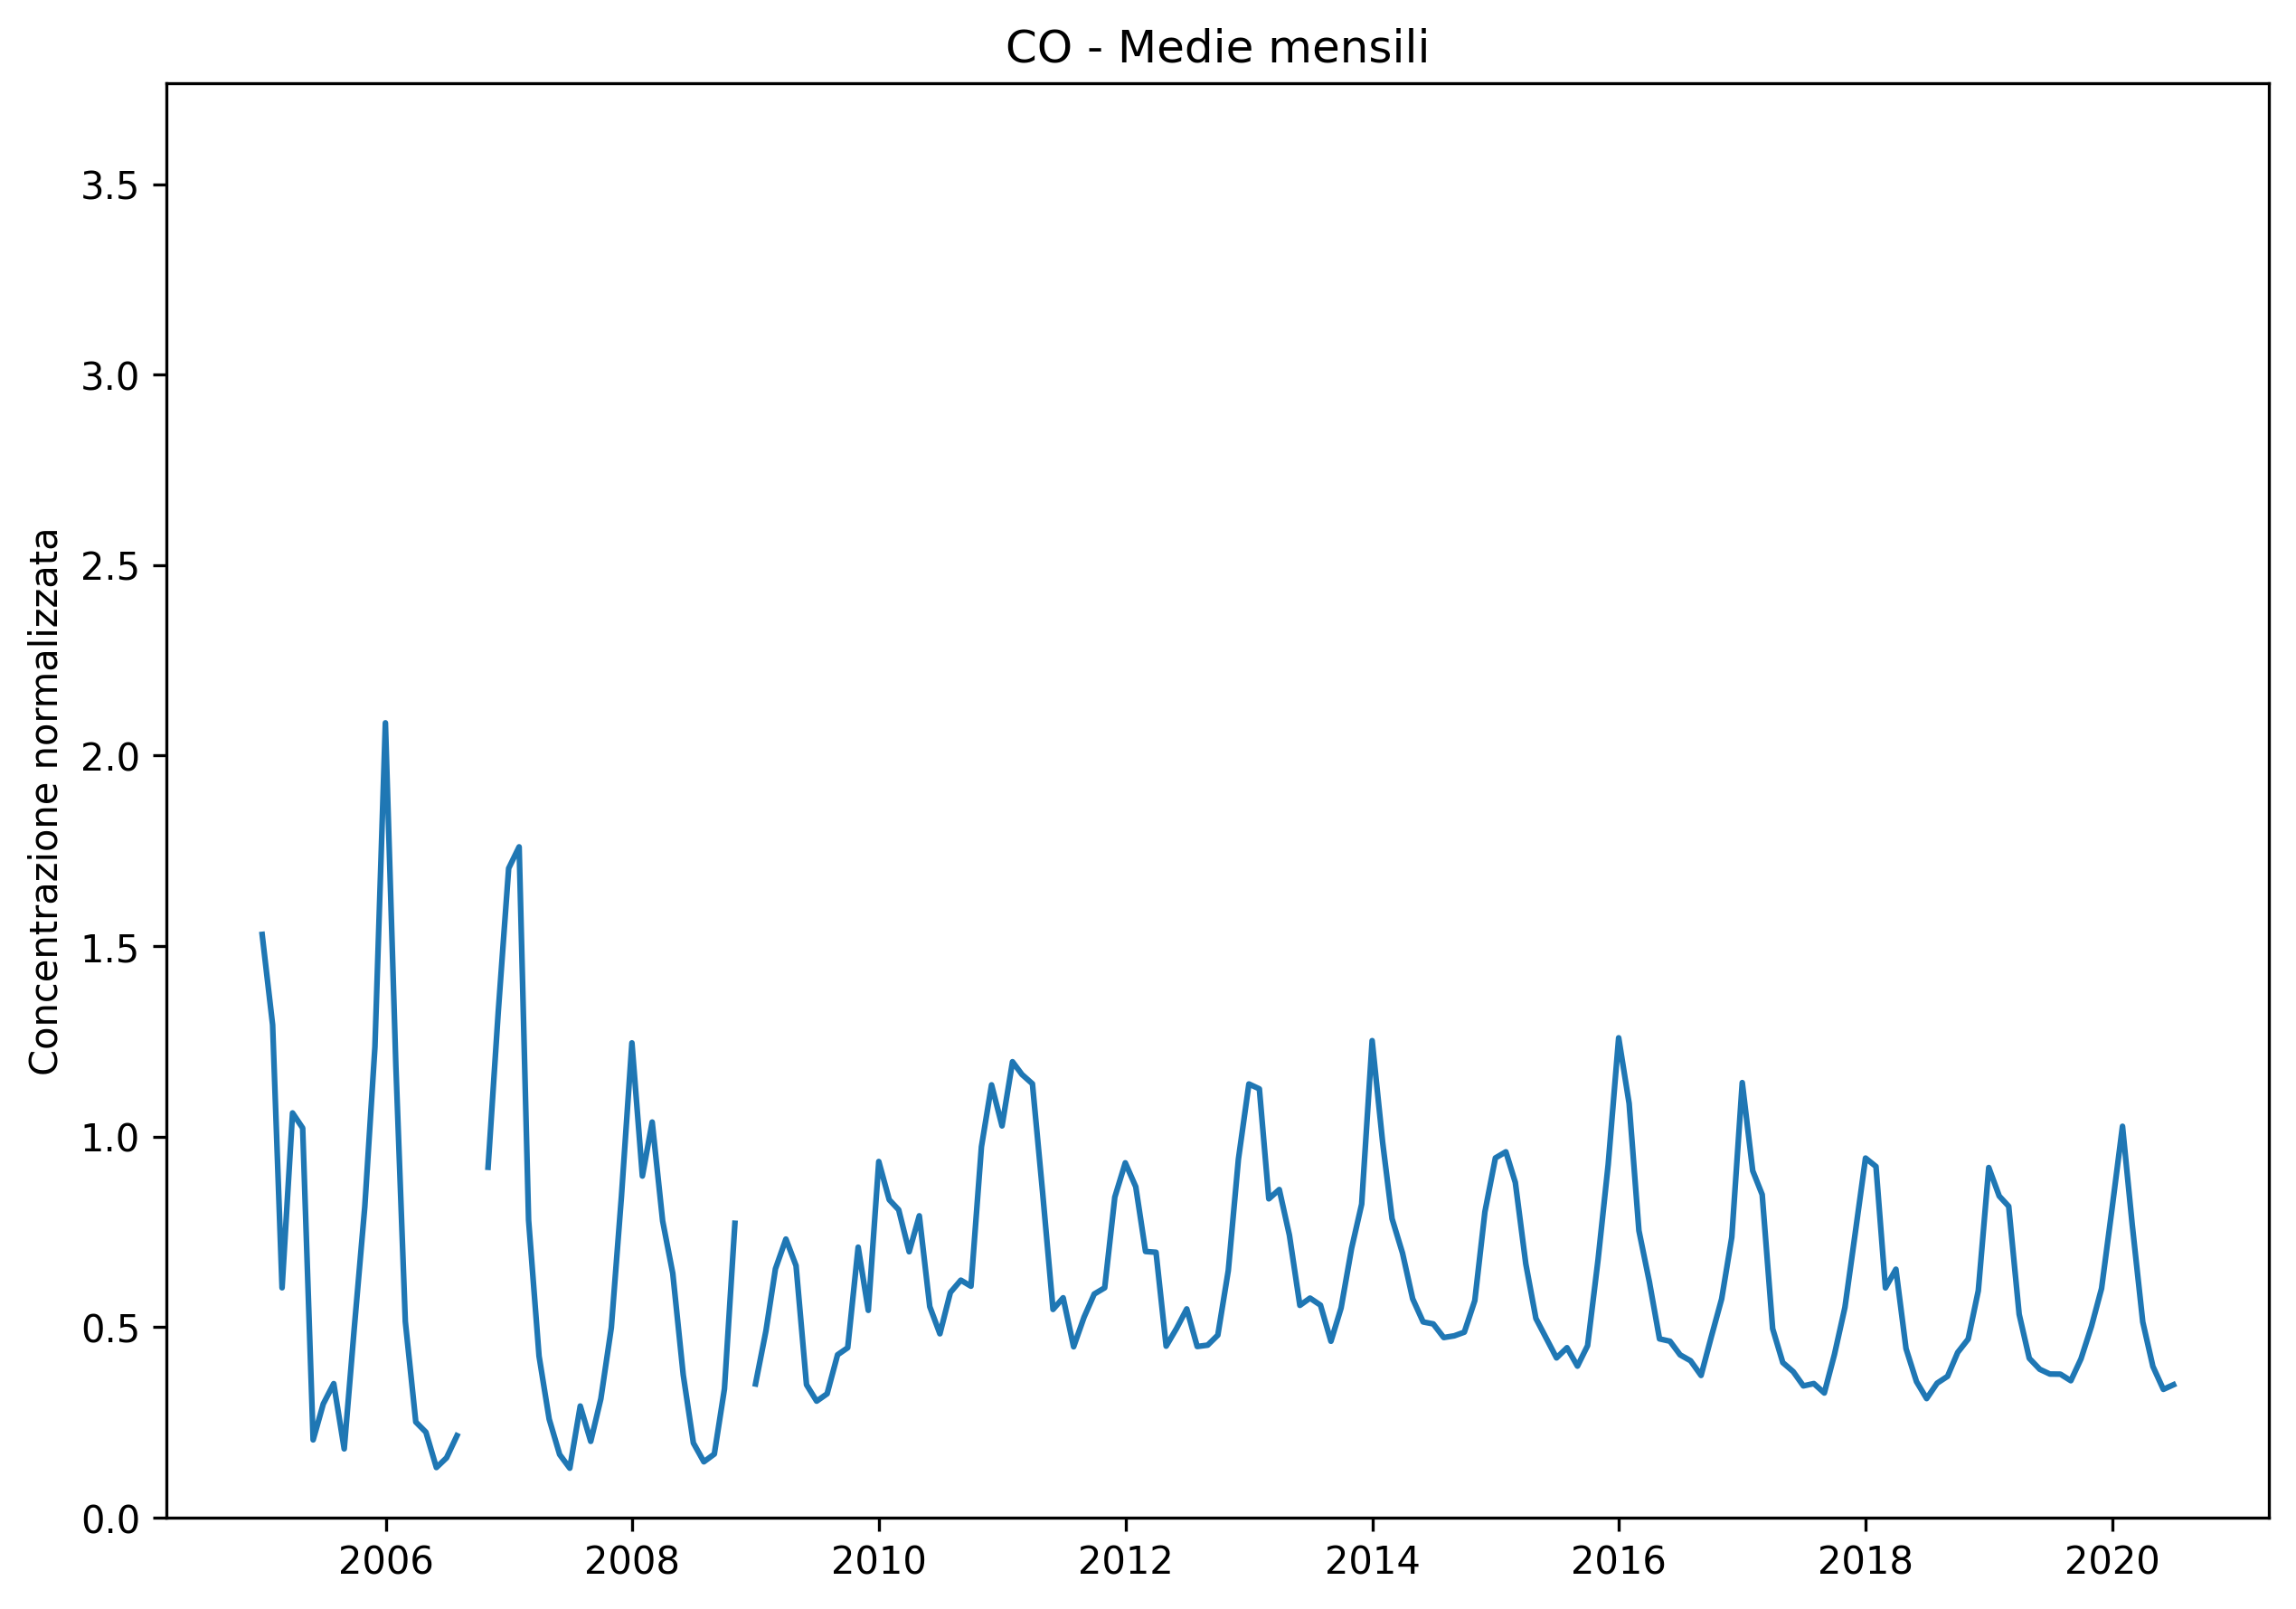
\includegraphics[width=0.75\textwidth]{CO_medie_mensili}
\caption{Medie mensili CO}
\label{fig:co_medie_mensili_reali}
\end{figure}

\begin{figure}
\centering
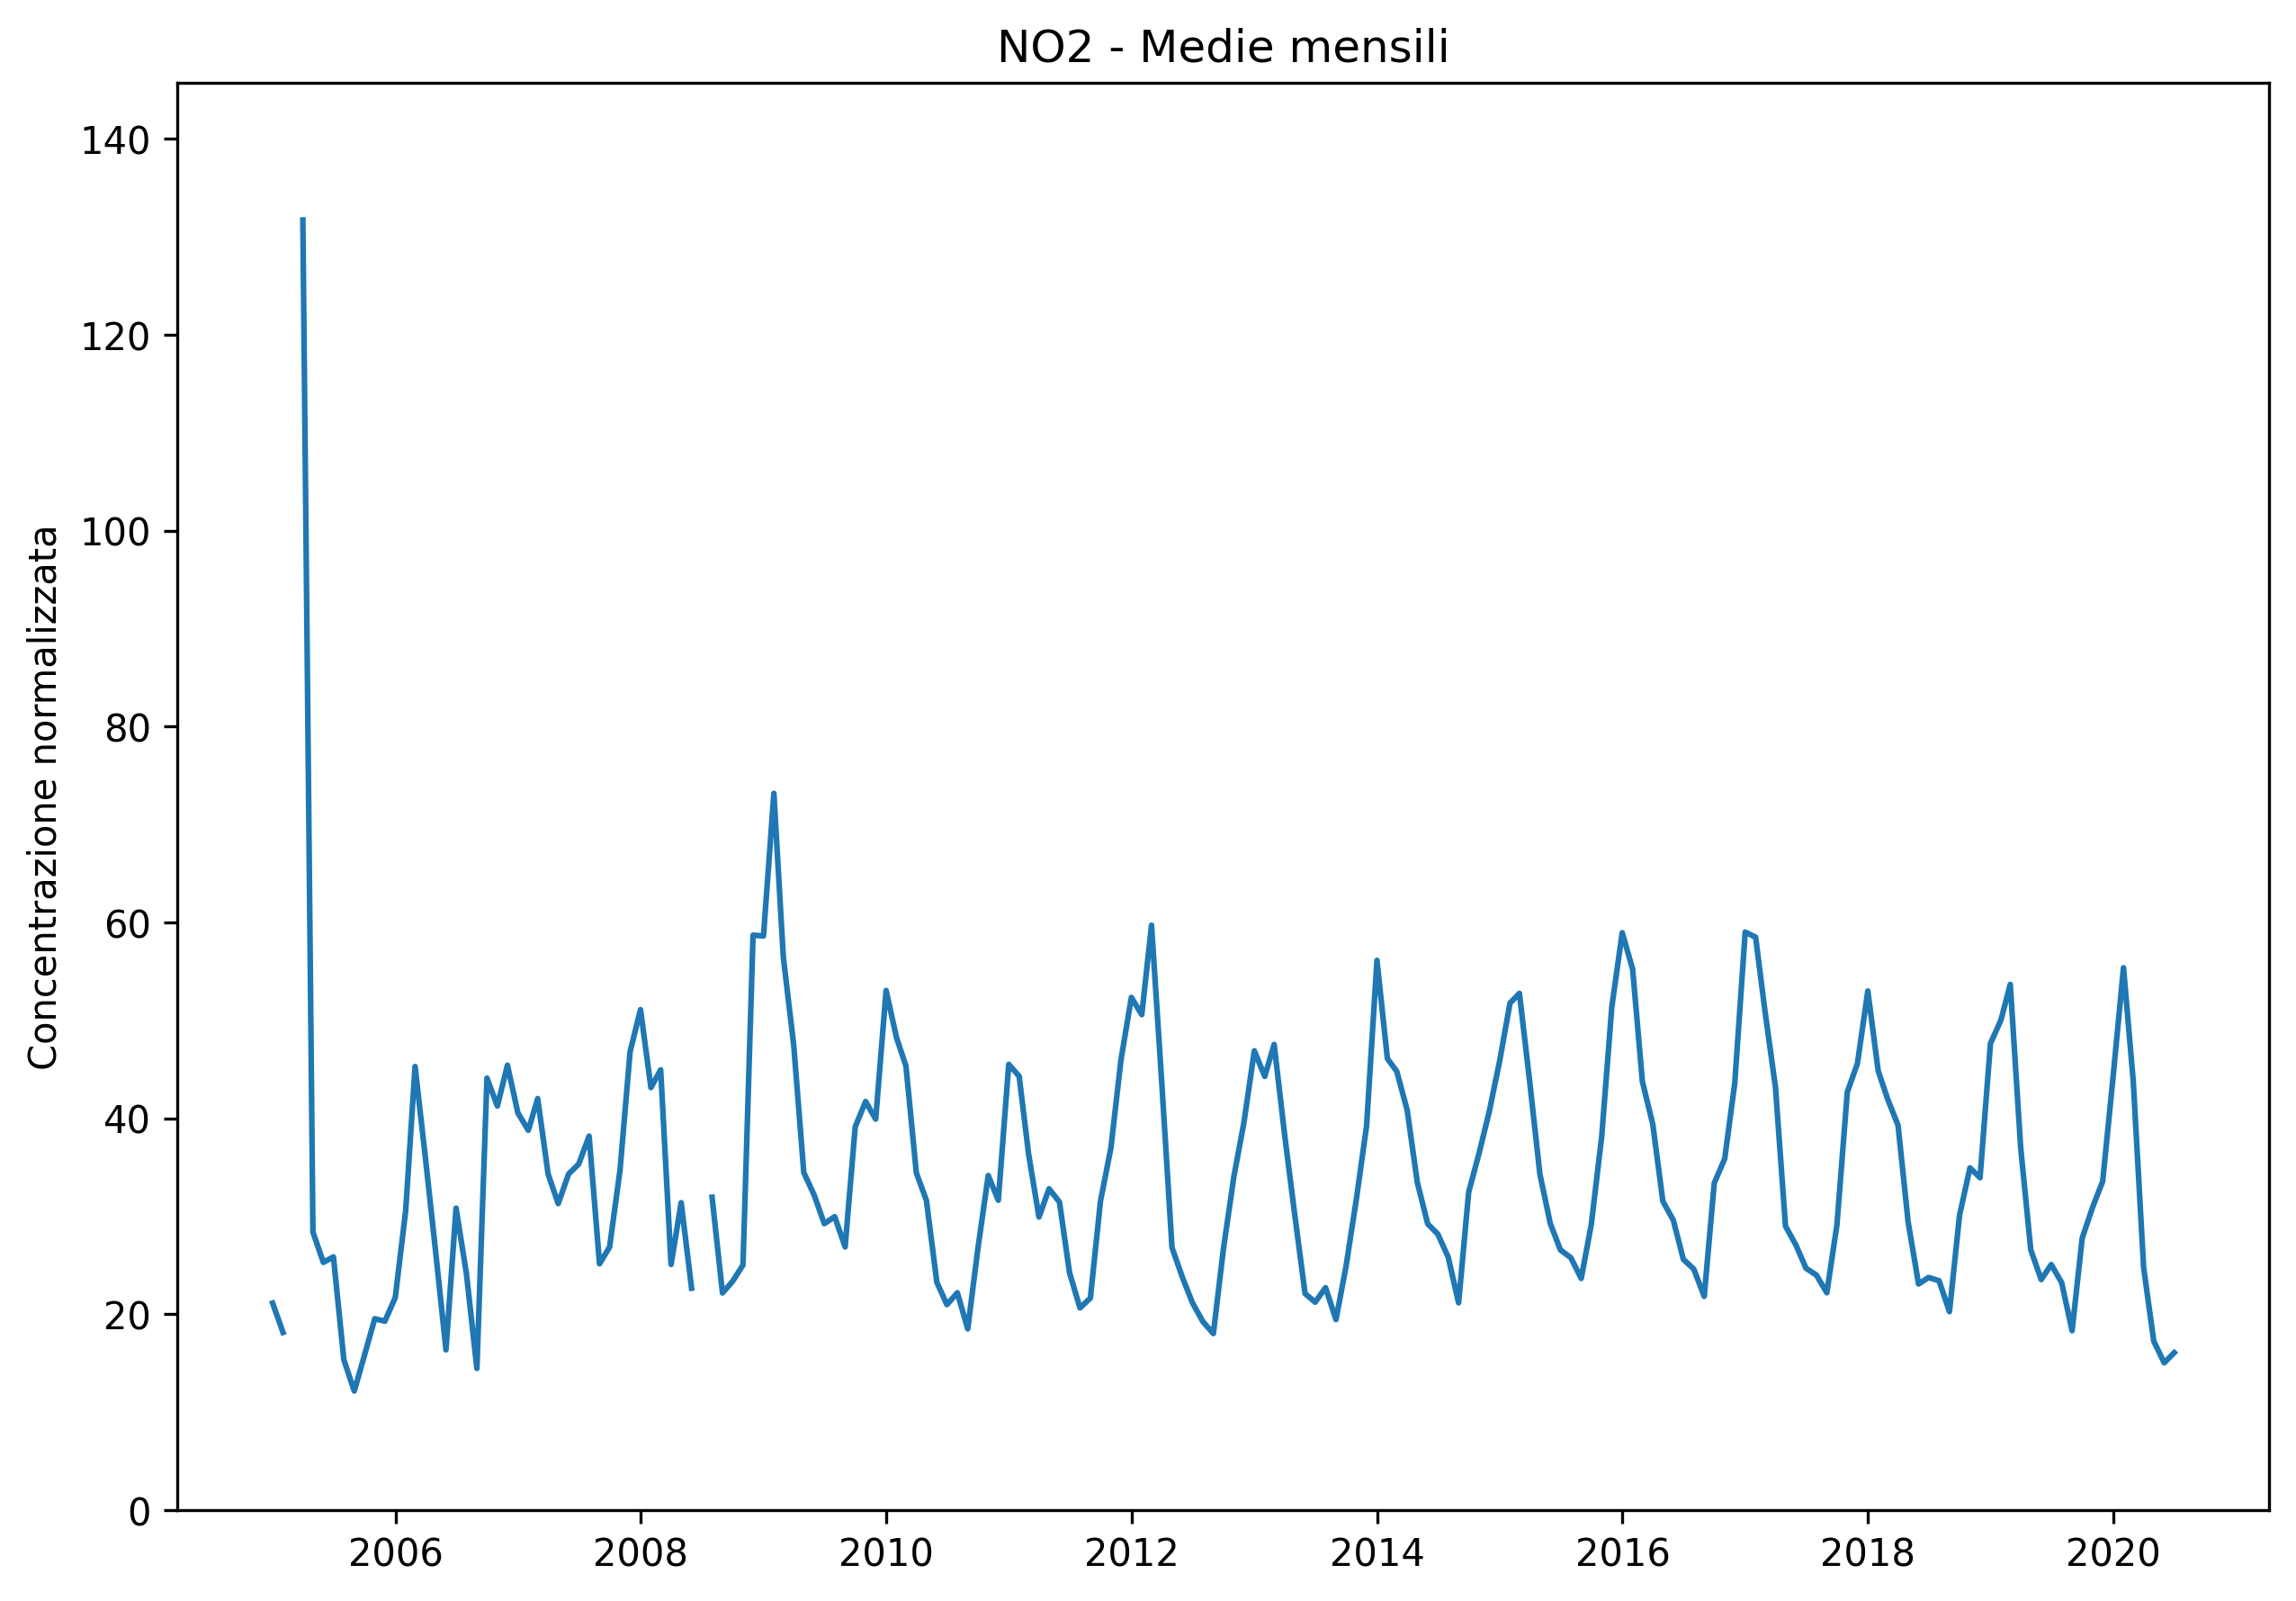
\includegraphics[width=0.75\textwidth]{NO2_medie_mensili}
\caption{Medie mensili NO2}
\label{fig:no2_medie_mensili_reali}
\end{figure}

\begin{figure}
\centering
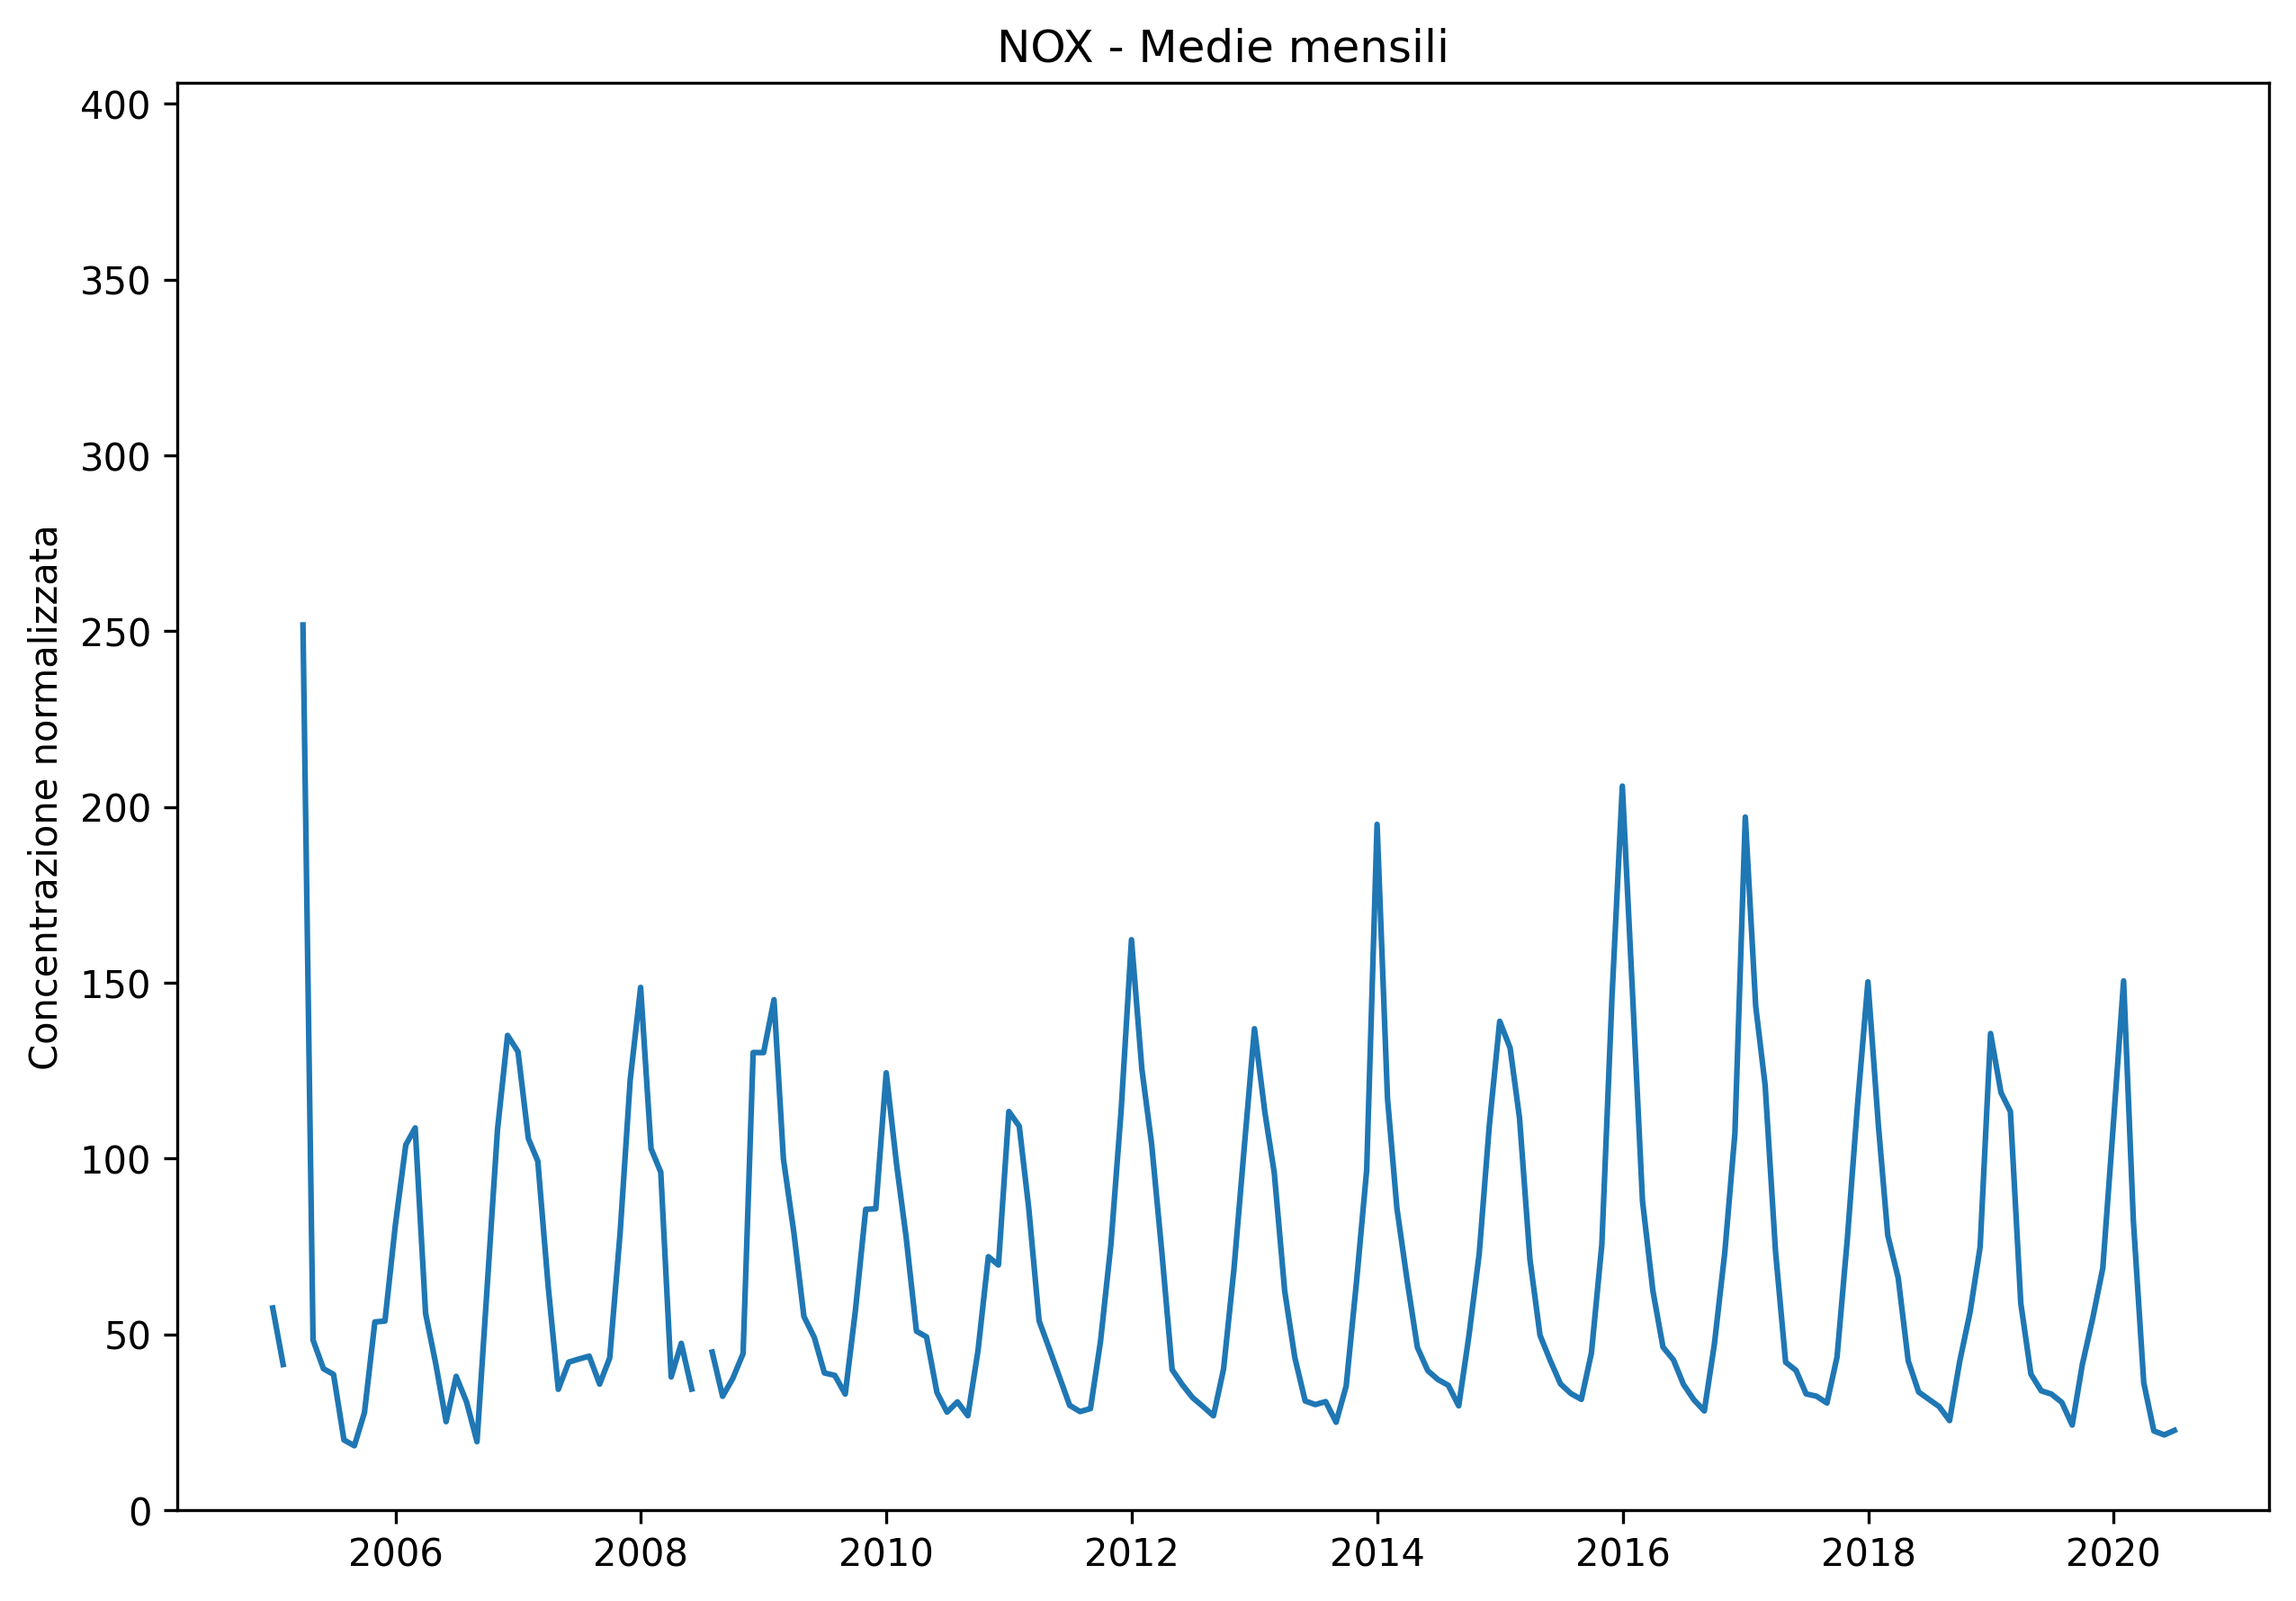
\includegraphics[width=0.75\textwidth]{NOX_medie_mensili}
\caption{Medie mensili NOX}
\label{fig:nox_medie_mensili_reali}
\end{figure}

\begin{figure}
\centering
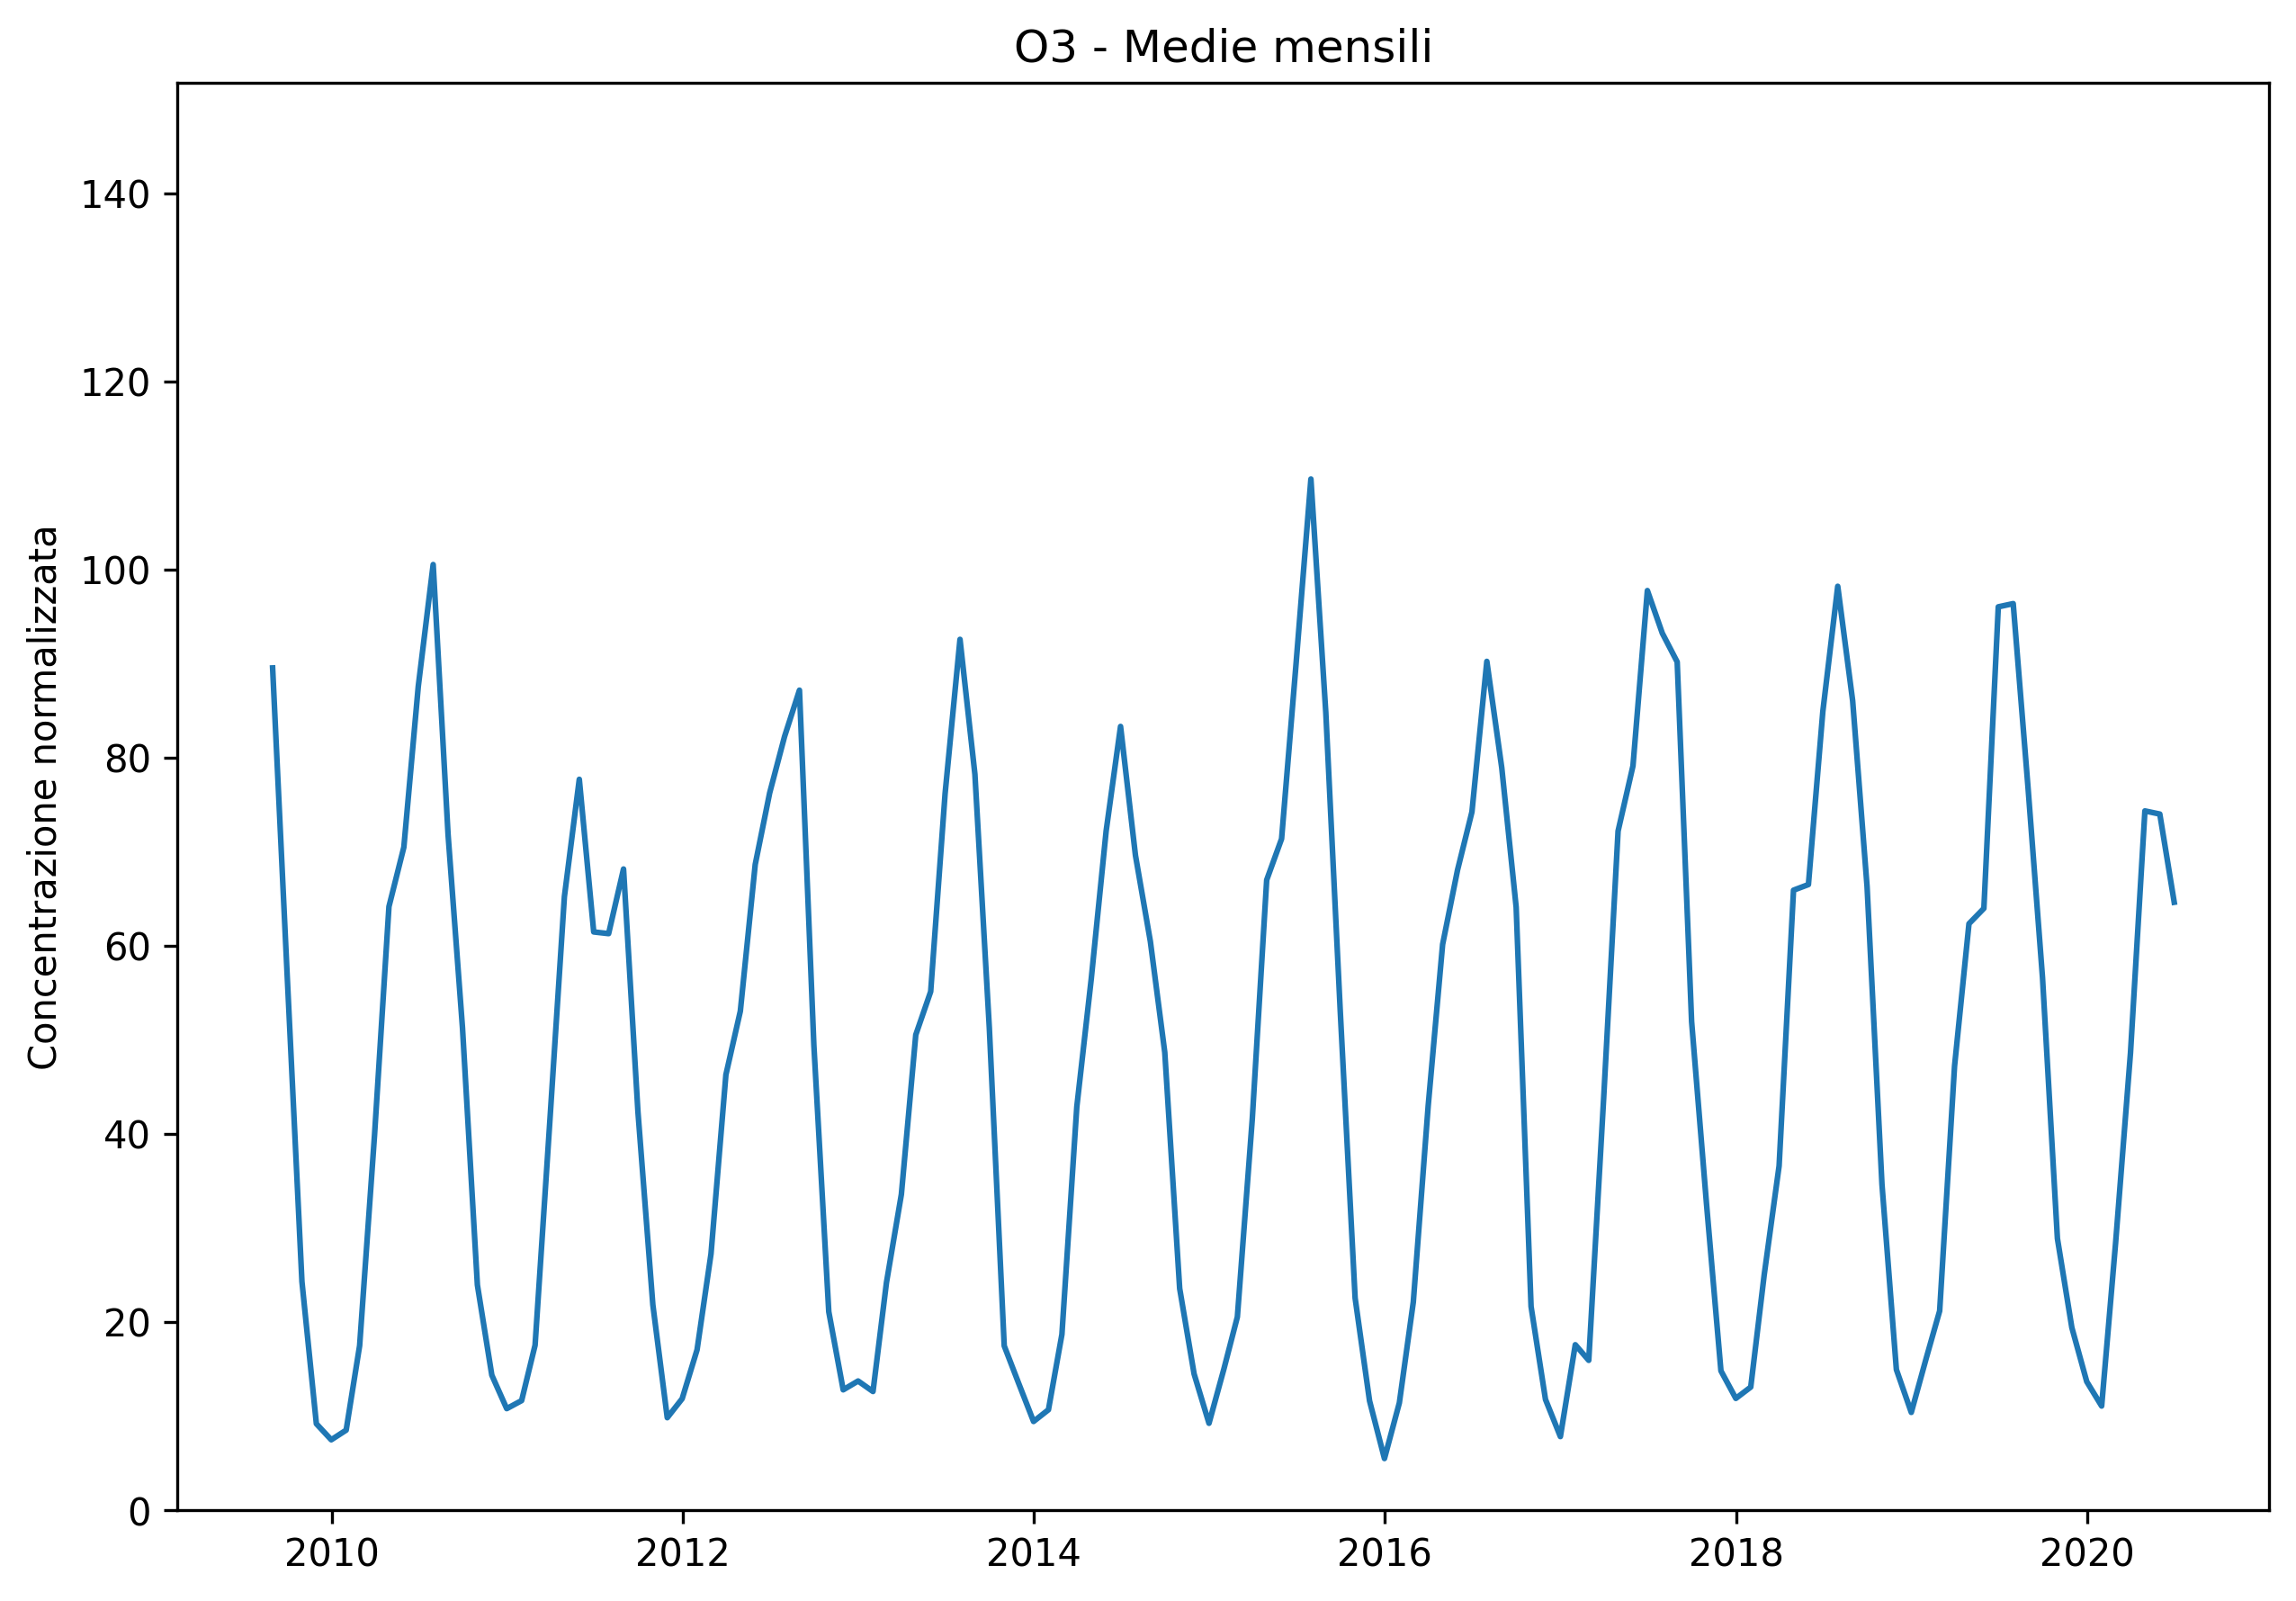
\includegraphics[width=0.75\textwidth]{O3_medie_mensili}
\caption{Medie mensili ozono}
\label{fig:o3_medie_mensili_reali}
\end{figure}

\begin{figure}
\centering
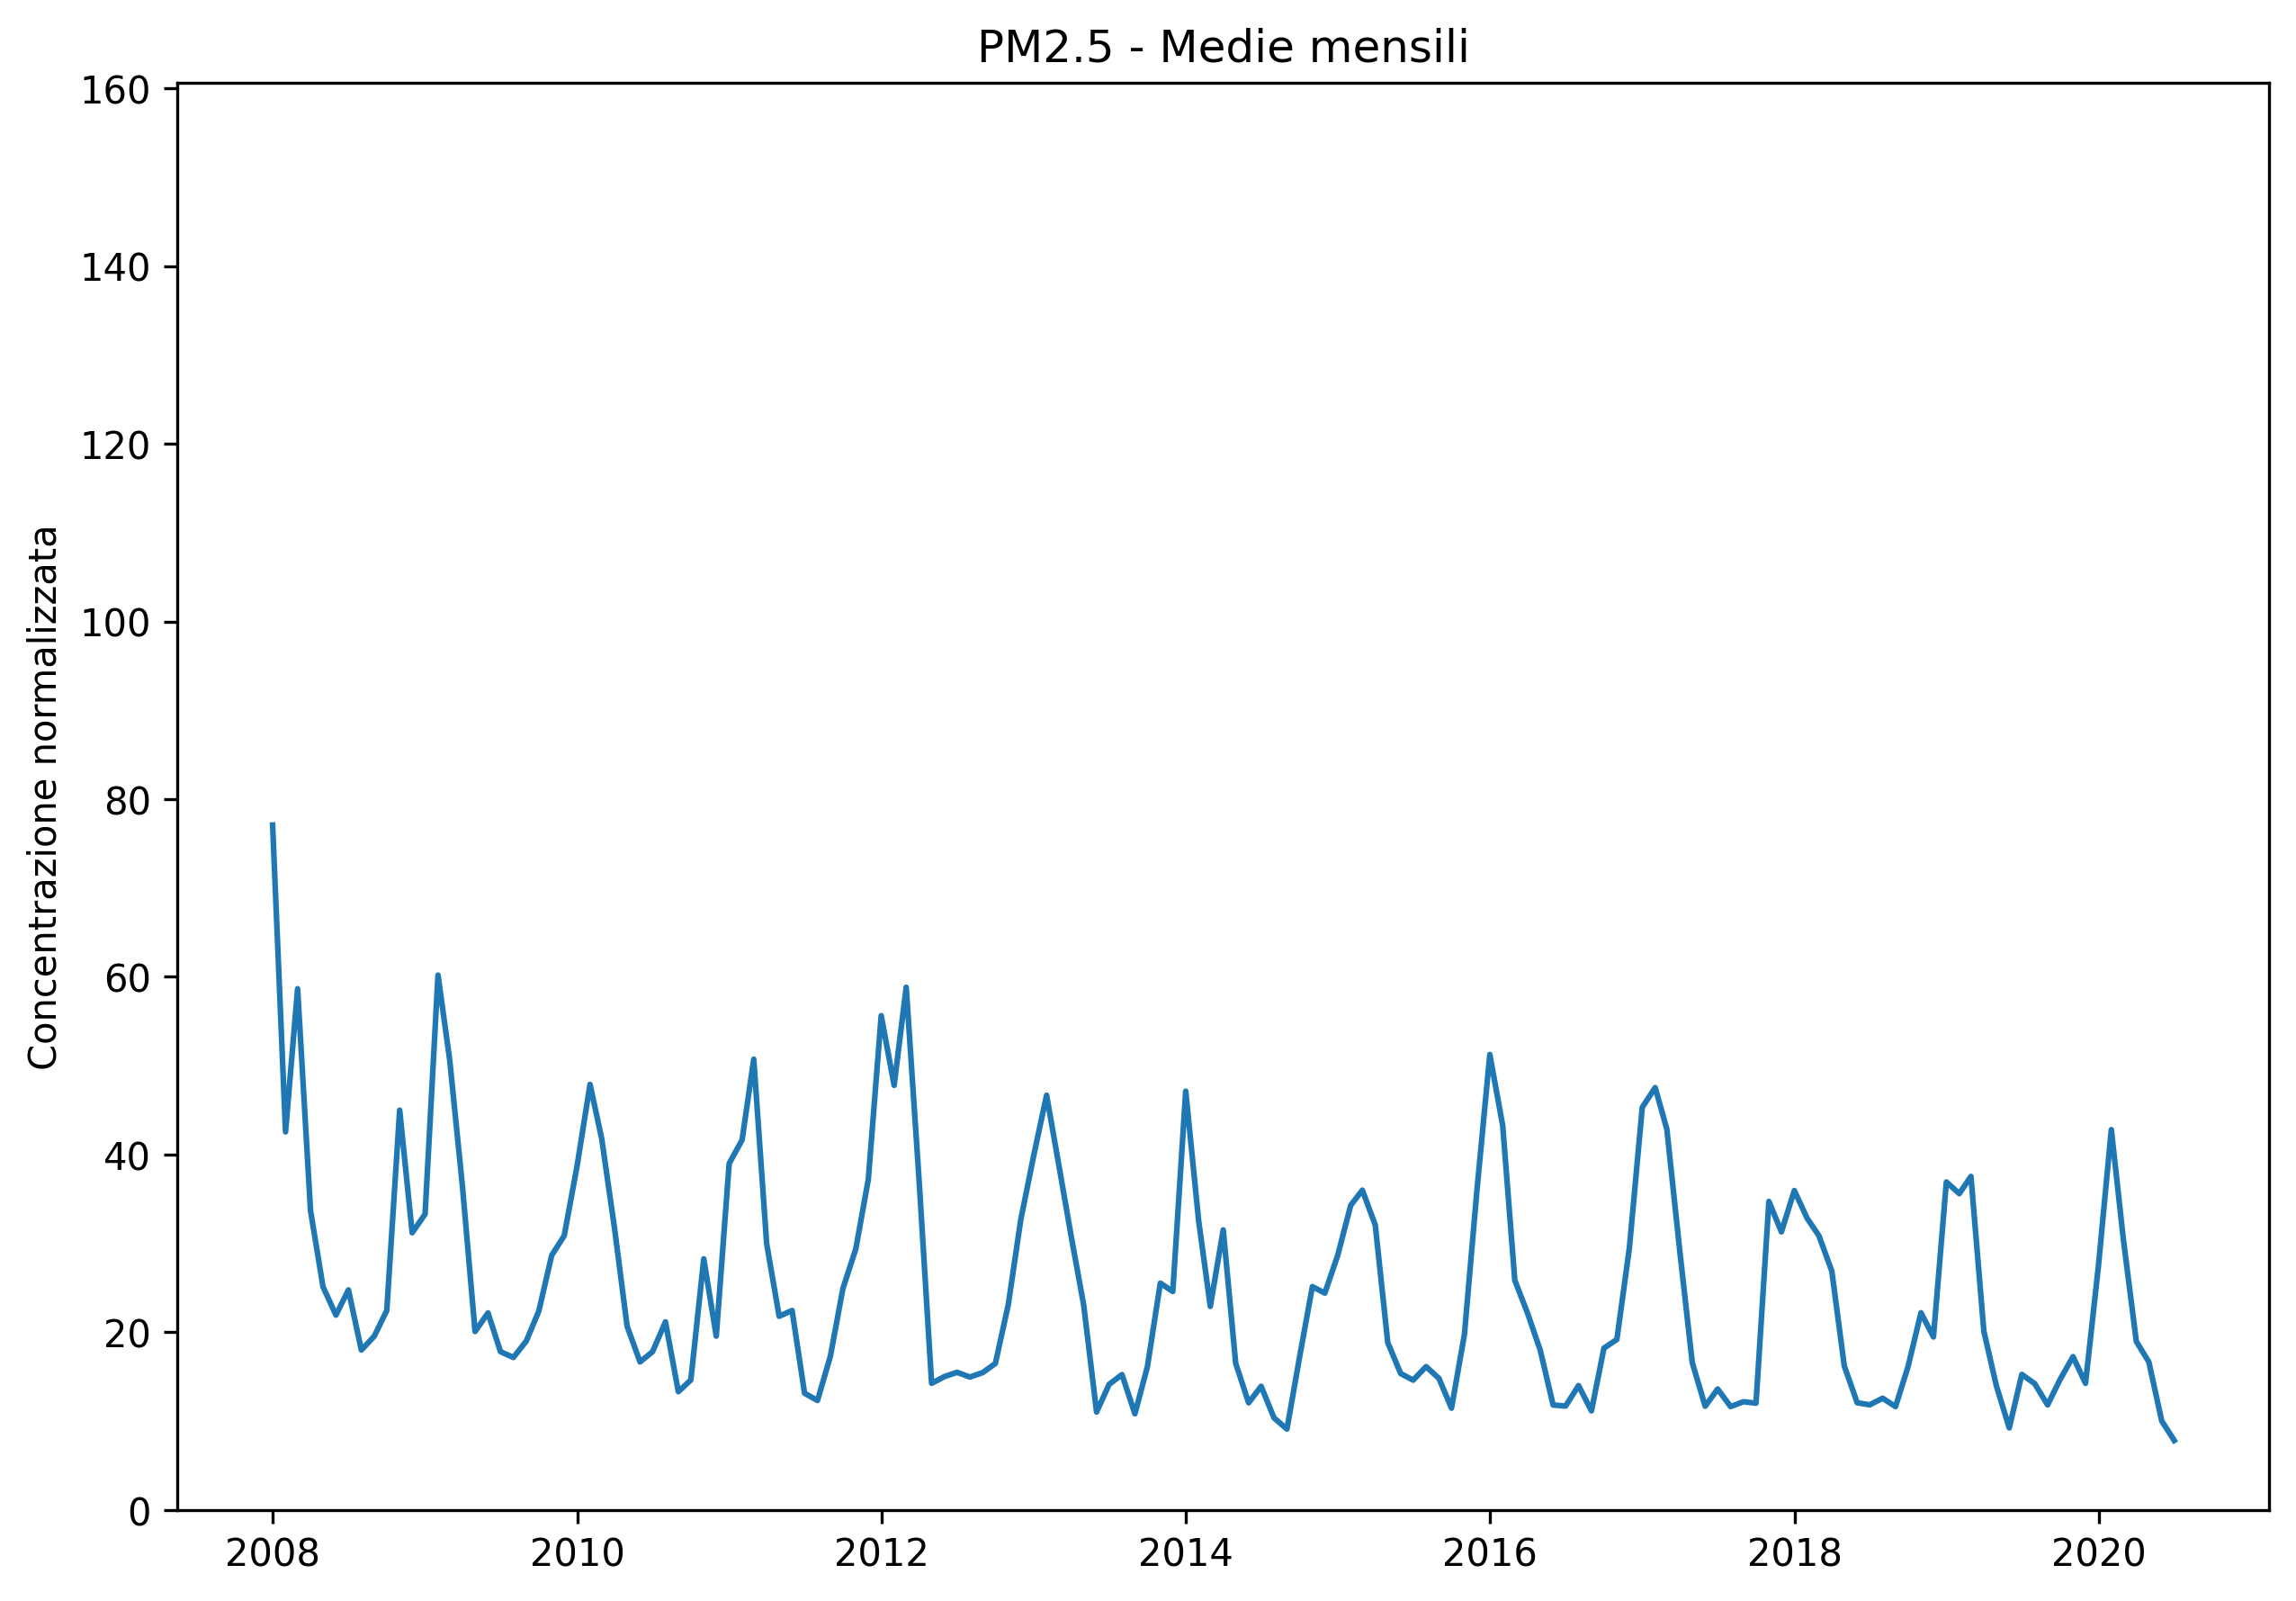
\includegraphics[width=0.75\textwidth]{PM2.5_medie_mensili}
\caption{Medie mensili PM2.5}
\label{fig:pm25_medie_mensili_reali}
\end{figure}

\begin{figure}
\centering
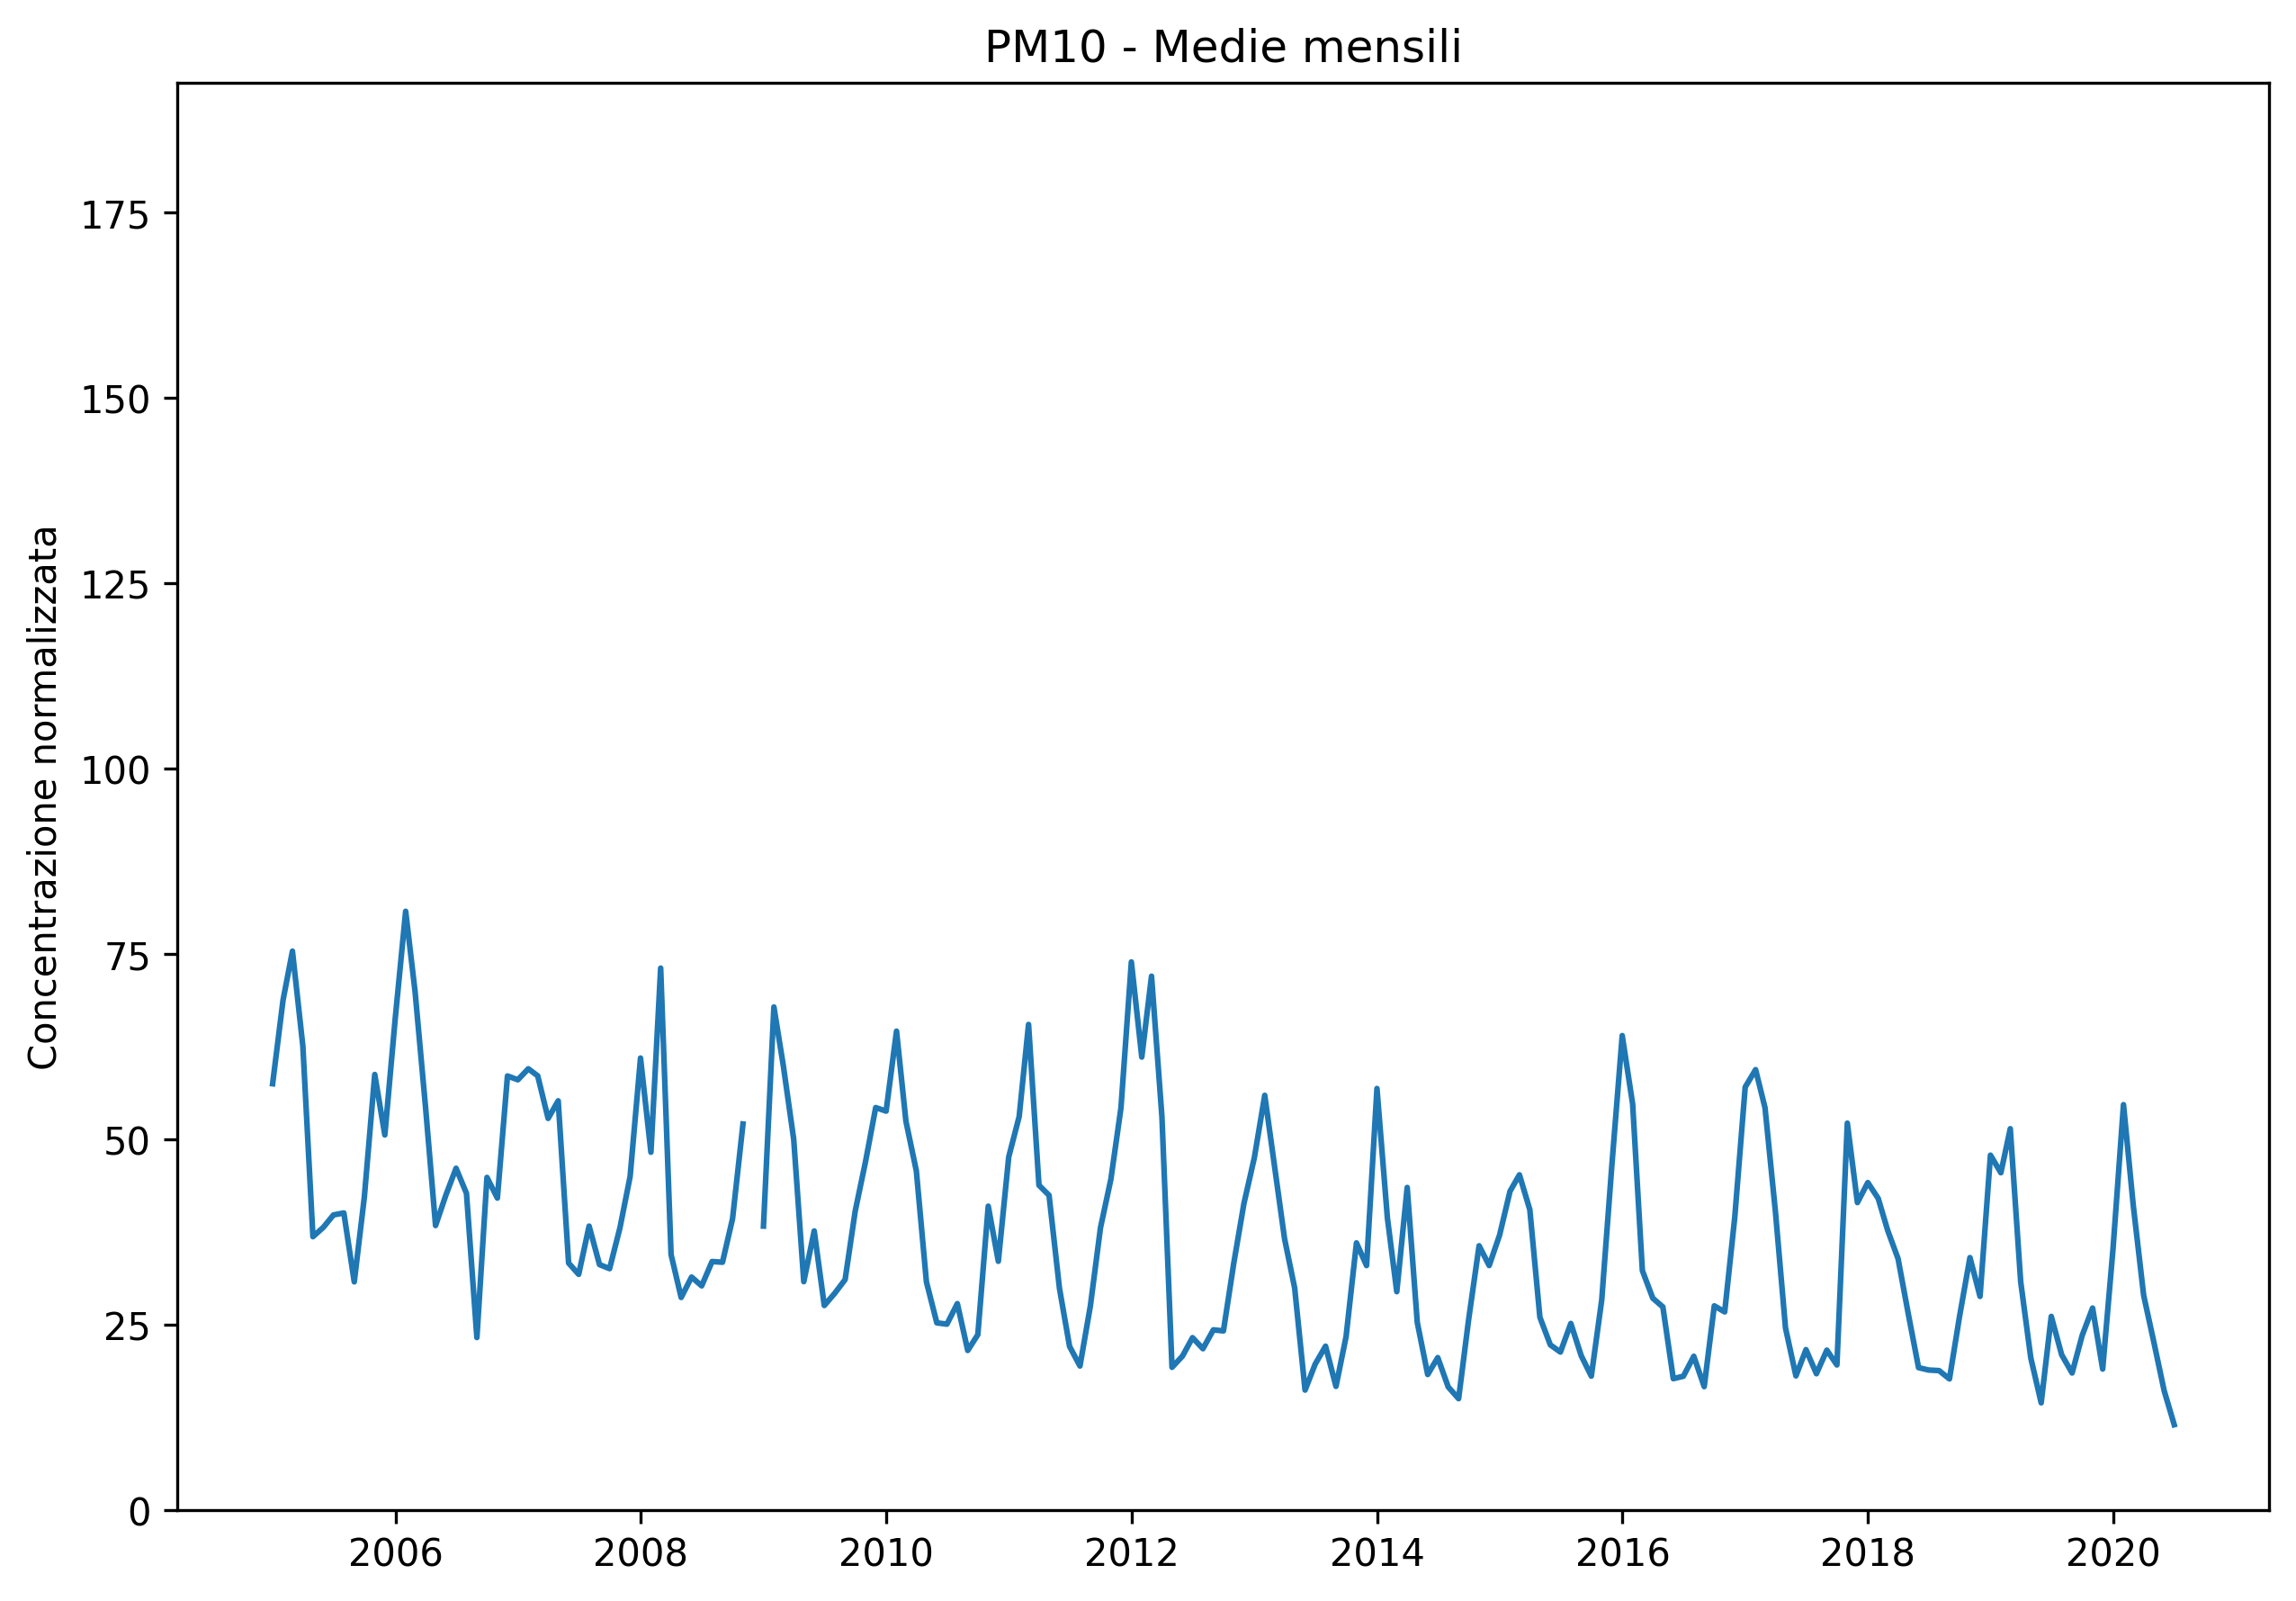
\includegraphics[width=0.75\textwidth]{PM10_medie_mensili}
\caption{Medie mensili PM10}
\label{fig:pm10_medie_mensili_reali}
\end{figure}

\begin{figure}
\centering
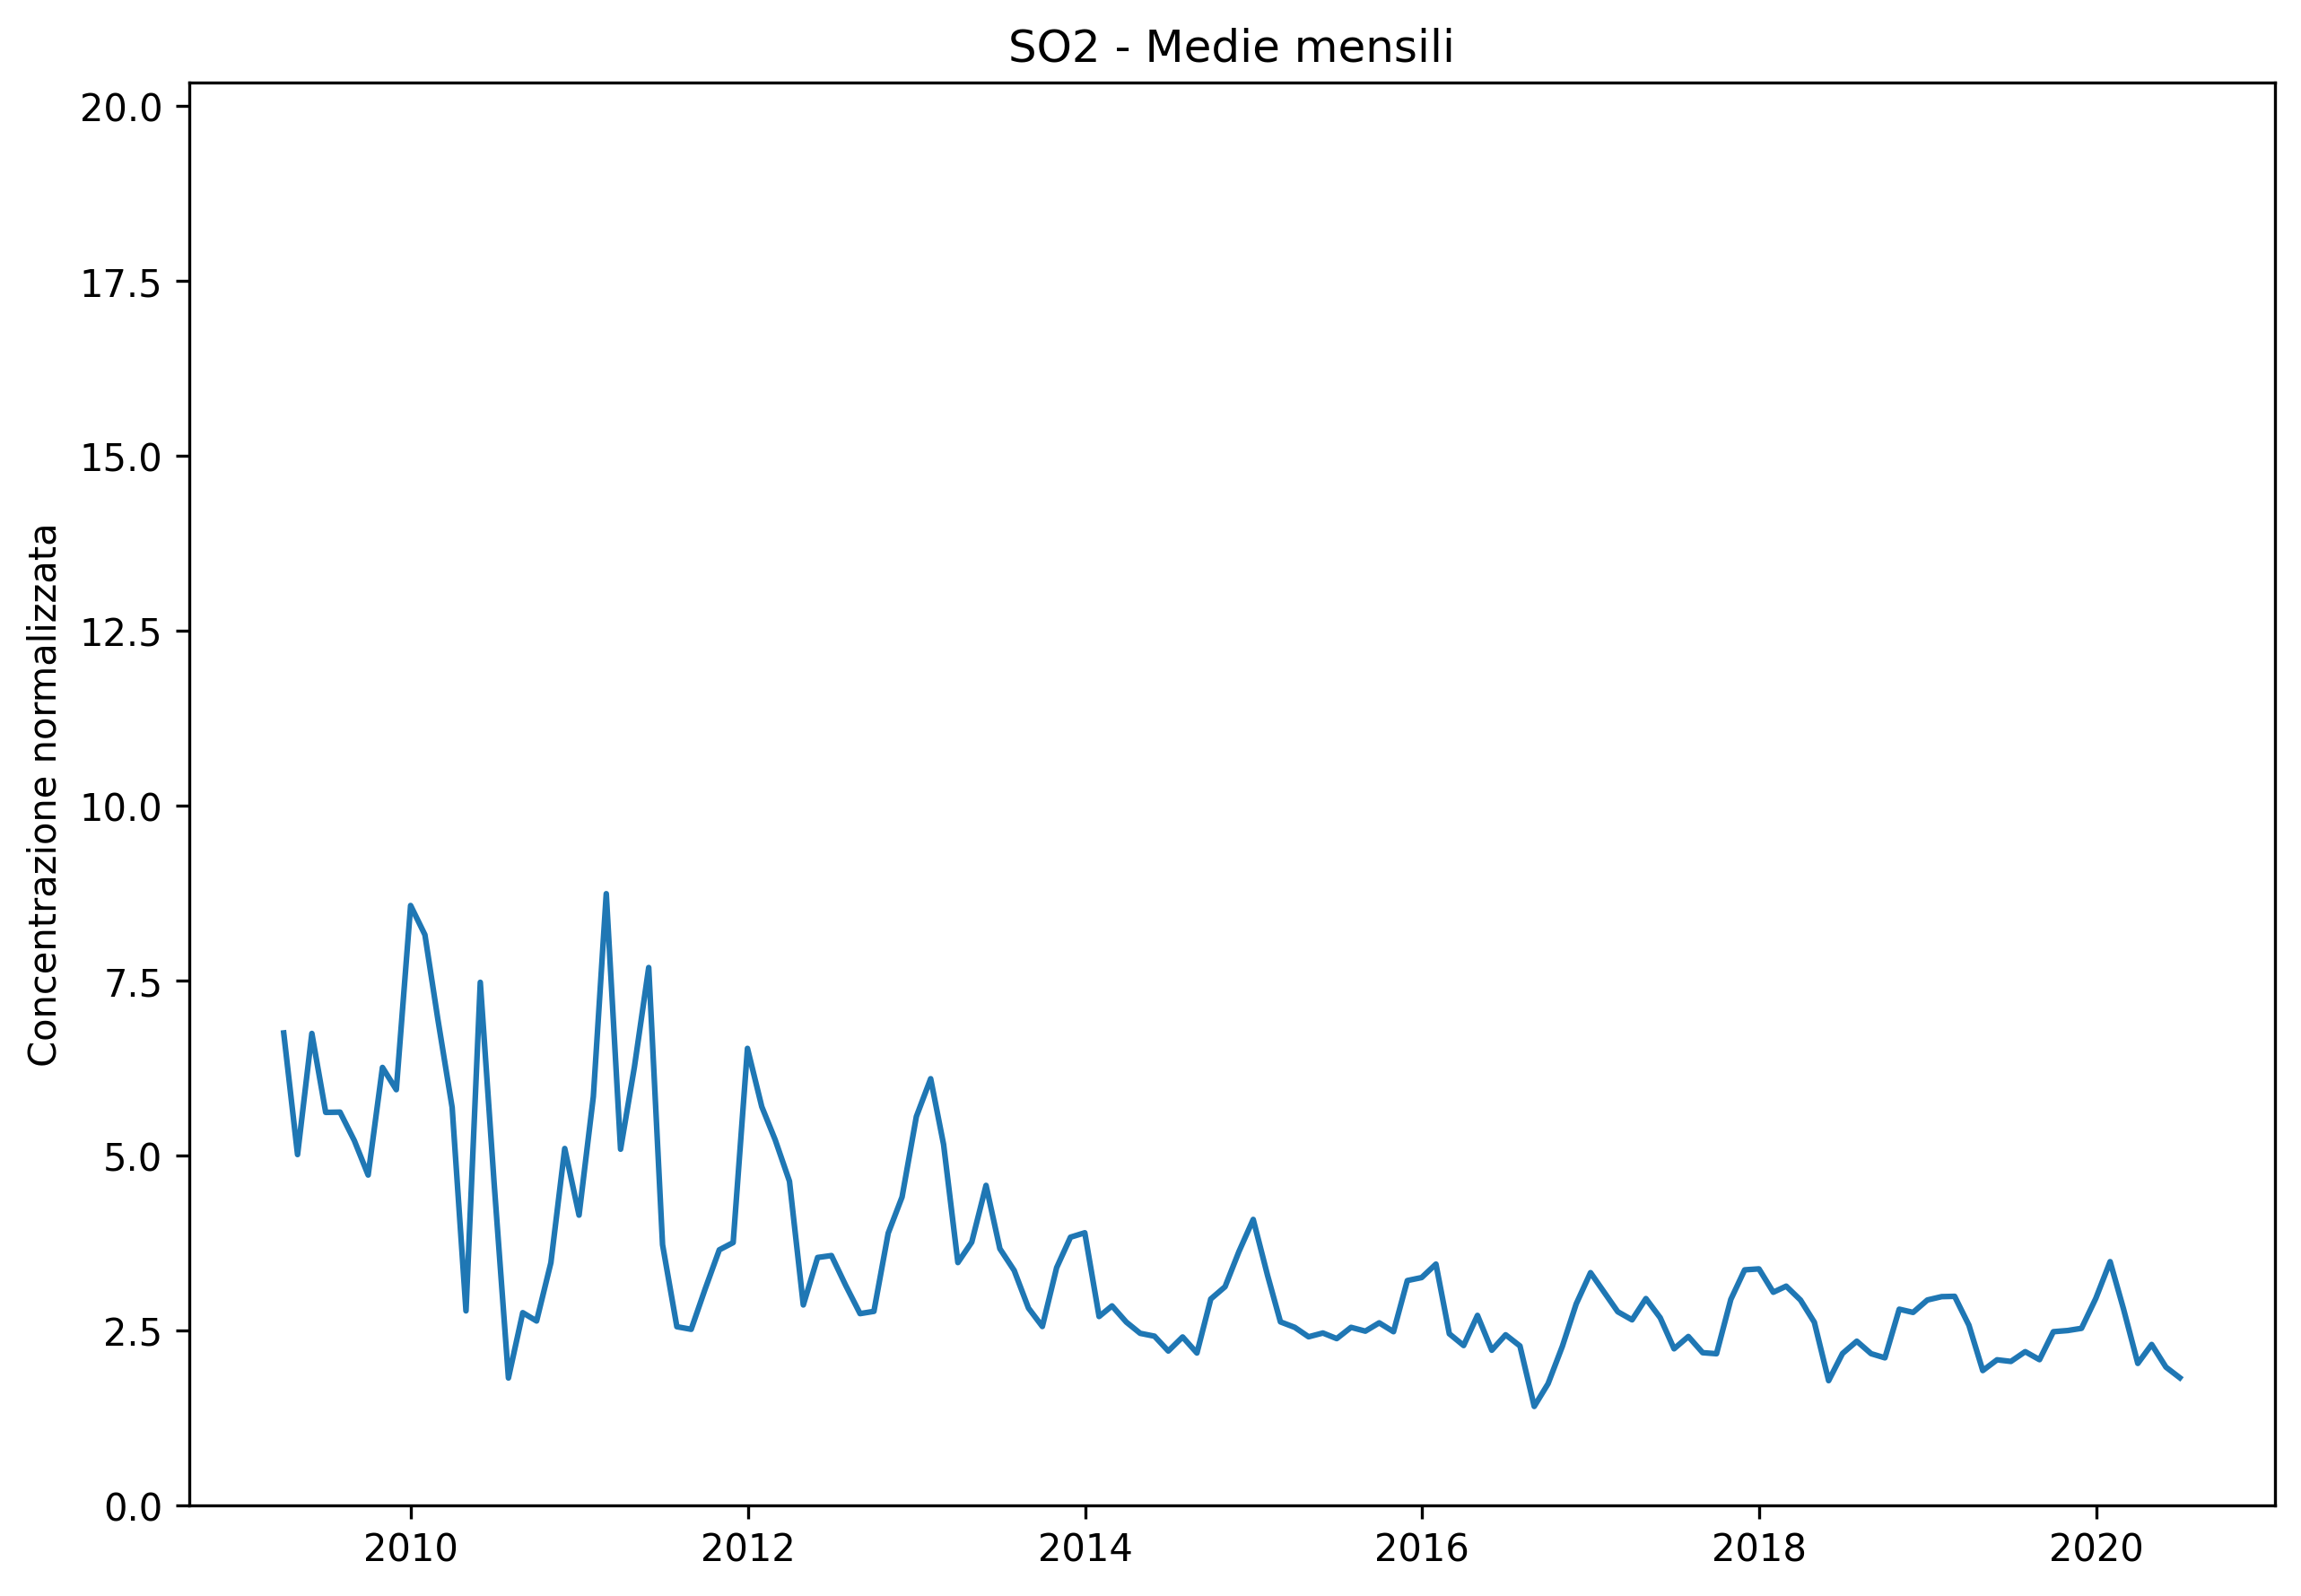
\includegraphics[width=0.75\textwidth]{SO2_medie_mensili}
\caption{Medie mensili SO2}
\label{fig:so2_medie_mensili_reali}
\end{figure}
